
%% Call for Papers
%% ExaMPI20 - Workshop on Exascale MPI 2020
%% Sunday, November 15th, 2020
%% Atlanta, GA, USA
%% 
%% Held in conjunction with SC20:  The International Conference for High
%% Performance Computing, Networking, Storage and Analysis 
%% 
%% In cooperation with the IEEE Computer Society Technical Consortium on
%% High Performance Computing (TCHPC)
%% 
%% The MPI standard and its implementations have proved surprisingly
%% scalable. Issues that hampered scalability have been addressed in the
%% MPI 2.1 – 2.2 definition process, and continued into MPI 3.0 and
%% 3.1. Thus, MPI has been robust and has been able to evolve, without
%% fundamentally changing the model or specification. For this and many
%% other reasons, MPI is currently the de-facto standard for HPC systems
%% and applications. However, there is a need for re-examination of the
%% message-passing model for extreme-scale systems characterized by
%% asymptotically decreasing local memory and highly localized
%% communication networks. Likewise, there is a need for exploring new
%% innovative and potentially disruptive concepts and algorithms
%% partially to explore other roads than those taken by the recently
%% released MPI 2018 Draft Specification. The aim of this workshop is to
%% bring together developers and researchers to present and discuss
%% innovative algorithms, protocols, operations, and concepts in Message
%% Passing programming models, in particular related to MPI or MPI+X. 
%% 
%% 
%% Topics of interest include (but are not limited to):
%% 
%% ·       Design and development of scalable Message Passing collective operations.
%% ·       Communication and architecture topology mapping interfaces and algorithms.
%% ·       Innovative algorithms for scheduling/routing to avoid network congestion.
%% ·       Integrated use of structured data layout descriptors.
%% ·       One-sided communication models and RDMA-based MPI.
%% ·       Support for heterogenous compute devices and heterogeneous memory systems.
%% ·       MPI multi-threading and threading requirements from OSes.
%% ·       Interoperability of Message Passing and PGAS models.
%% ·       Integration of task-parallel models into Message Passing models.
%% ·       Fault tolerance in MPI.
%% ·       MPI I/O.
%% 
%% Paper submission and publication
%% ---------------------------------------------------------------------------------------
%% There are two submission categories:
%% 
%% ·    Regular research paper: submission of full paper. Regular paper
%% submissions are limited to 10 single-space pages (including figures,
%% tables and references) using a 10-point on 8.5x11-inch pages (US
%% Letter). 
%% 
%% Templates can be found at:
%% http://www.ieee.org/conferences_events/conferences/publishing/templates.html. Instructions
%% for preparing regular papers for the proceedings will be emailed to
%% authors of accepted papers. Submitted regular papers will be
%% peer-reviewed and accepted papers will be published by the IEEE TCHPC.
%% 
%% Important dates
%% ---------------------------------------------------------------------------------------
%% Paper Submissions Deadline: August 31, 2020
%% Paper Notification: September 28, 2020
%% Final Camera Ready Version: October 5, 2020

\documentclass[conference,10pt,letterpaper]{IEEEtran}

\usepackage{graphicx}
\usepackage{balance}
\usepackage{url}
%
\usepackage{todonotes}% who needs this?
%
\long\def\comment#1{}
%
\begin{document}

\title{MPI International Survey Report}

\author{
  \IEEEauthorblockN{Atsushi Hori}
  \IEEEauthorblockA{Riken Center for Computational Science\\
    Email: ahori@riken.jp}
  \and
  \IEEEauthorblockN{Jie Yin}
  \IEEEauthorblockA{Riken Center for Computational Science\\
    Email: jie.yin@riken.jp}
  \and
  \IEEEauthorblockN{Takahiro Ogura}
  \IEEEauthorblockA{Riken Center for Computational Science\\
    Email: t-ogura@riken.jp}
  \and
  \IEEEauthorblockN{Balazs Gerofi}
  \IEEEauthorblockA{Riken Center for Computational Science\\
    Email: bgerofi@riken.jp}
  \and
  \IEEEauthorblockN{George Bosilca}
  \IEEEauthorblockA{The University of Tennessee, Knoxville\\
    Email: bosilca@icl.utk.edu}
  \and
  \IEEEauthorblockN{Emmanuel Jeannot}
  \IEEEauthorblockA{Inria\\
    Email: emmanuel.jeannot@inria.fr}
  \and
  \IEEEauthorblockN{Yutaka Ishikawa}
  \IEEEauthorblockA{Riken Center for Computational Science\\
    Email: yutaka.ishikawa@riken.jp}
}  

\maketitle

\begin{abstract}
-- this abstract should be rewritten --
%
The Message Passing Interface (MPI) plays a critical part in the
parallel computing ecosystem, a driving force behind many of the
high-performance computing (HPC) successes. To maintain its relevance
to the user community---and in particular to the growing HPC community
at large---the MPI standard needs to identify and understand the MPI
users' expectations and concerns, and adapt accordingly.
%
% Our survey is international and targets novice to expert
% users, hoping to be a complement to the ECP survey.

This survey was conducted from February, and at the time of
this writing has gathered more than 800 answers from 42 countries.
%
This report, based the July 2020 results of the survey,
focuses on the MPI users communities awareness of MPI features.
% which MPI features MPI users know and which ones they do not.
%
%This survey reveals the staggering fact that most MPI users make use
%of a small subset of the MPI API, a subset that mostly avoids features
%introduced after MPI 2.2, released in 2009, such as PMPI, dynamic
%process creation, and persistent communications. Further, the survey
%reveals that many MPI users learn MPI from the internet and/or some
%form of online documents, highlighting a shift in the education of the
%target community.
%
%These two outcomes seem to suggest that many MPI users failed to receive the
%information about new MPI features because most internet sources are outdated
%and lack support for them. It also suggests that one quick way to address this
%is to provide the necessary education, possibly as part of the MPI Forum effort.
\end{abstract}

\section{Background}

Existing studies on MPI uses are focused on a restricted target domain,
such as the Exascale Computing Project (ECP)~\cite{ECP} study
conducted in 2017~\cite{osti_1462877} that focused 
on MPI usage in the context of ECP applications; and/or those that are
geographically constrained to a single laboratory, funding agency or
at best, country. It ws a coincidence
that another survey was conducted in Japan targeting HPCI\cite{HPCI}
users which included several questions asking about
MPI\cite{hpci-user-survey}.  HPCI is an infrastructure for HPC users
in Japan connecting major supercomputers owned by universities and
governmental research institutes. If both questionnaire surveys would
have the same questions, then we could compare the answers to reveal
the differences between US and Japan. Unfortunately we could find only
one similar question related to MPI in both surveys.
%
Such studies inspired us to conduct a larger study, not focused on
high-end HPC, but targeting a wider audience and involving a larger
spectrum of geographically distinct users. Since MPI has been a widely
used vehicle for high-performance computing for decades, this
larger-scale questionnaire survey would be beneficial not only for
deciding the future direction of MPI, but also for understanding the
feature differences of MPI users among countries and/or regions of the
world.
%
Our project was started to conduct such a study as a part of
JLESC\cite{JLESC} which is an international research collaboration
framework. The international nature of this survey matches the concept
of JLESC. Co-authors are a member of JLESC and responsible for the
country and/or region where he belongs. On the design a questionnaire,
we consulted two social scientists, Prof. Marshall Scott Poole at
Illinois Univ., and Prof. Iftekhar Ahmed at Univ. of North Texas,
participating JLESC workshops to investigate how researchers can
cooperate in the JLESC framework. 
%
\begin{table}[htb]%
\begin{center}%
\caption{Survey Comparison}\label{tab:comparison}%
\begin{tabular}{c|cccc}%
\hline%
Name & Field of  & Geographic & Number of & Number of \\%
     & Interests & Target     & Questions & Participants \\%
\hline%
\hline%
ECP  & Exascale & US & 64 (max.) & 77 \\%
& Computing & & & \\%
\hline%
HPCI & Computing & Japan & 75 (max.) & 105 \\%
& Environment & & & \\%
\hline%
Ours & MPI & the globe & 30 & 851 \\%
\hline%
\end{tabular}%
\end{center}%
\end{table}%
%
Our MPI International Survey, ECP survey, and HPCI survey are
summarized in Table~\ref{tab:comparison}.
%
\comment{
The major differences
between our survey and the others are;

\begin{description}
\item[Geographic Target]\mbox{}\\
  The ECP survey targeted ECP members who are leading researchers and
  application developers in the US. The ECP survey targeted high-end
  users. Whereas our survey targets all MPI users from novices to experts.
\item[Number of participants]\mbox{}\\
  The number of participants of the ECP survey is 77. Because of the wider
  target of our survey, in terms of the scope of MPI expertise of
  participants on a global scale, the expected number of answers would
  be larger than those of preceding surveys.  
\item[Number of questions]\mbox{}\\
  The number of questions in our survey is 30 which is much
  smaller than those of the other surveys.
\end{description}
}

\section{Survey}
%
% Design
%
The social scientists suggested that the number of questions must be
limited around 30 not to reduce the participants' concentrations.  
This number is much smaller that those of ECP and HPCI surveys. So, we
focused on MPI communications and excluded MPI I/O related
questions. Additionally, we designed the questionnaire for
participants can easily answer questions as much as possible. As a
result, the questions to force participants doing some work, such as
counting the lines of code, are eliminated. Table~\ref{tab:questions}
lists all 30 questions.
%
ECP and our questionnaires are implemented by using Google Form. Later
in our project, we also implemented the same questionnaire by using
Microsoft Form for those who cannot access Google Form.
%
The draft questionnaire was tested by MPI Forum members and
researchers at Riken Center for Computational Science. 
The questionnaire was started distributing and receiving answers from
17th of February and it is still open.
%
\begin{table}
\begin{center}%
  \caption{Questions}\label{tab:questions}
\begin{tabular}{l|l}%
  \hline
  Q1  & What is your main occupation? \\
  \hline
  Coun- & Select main country or region of your workplace in past \\
  try & 5 years \\
  \hline
  Q2   & Rate your overall programming skill (non-MPI programs) \\
  \hline
  Q3   & Rate your MPI programming skill \\
  \hline
  Q4*  & What programming language(s) do you use most often? \\
  \hline
  Q5   & How long have you been writing computer programs \\
  & (incl. non-MPI programs)? \\
  \hline
  Q6   & How long have you been writing MPI programs? \\
  \hline
  Q7*  & Which fields are you mostly working in? \\
  \hline
  Q8*  & What is your major role at your place of work? \\
  \hline
  Q9   & Have you ever read the MPI standard specification \\
  & document? \\
  \hline
  Q10* & How did you learn MPI? \\
  \hline
  Q11* & Which MPI book(s) have you read? \\
  \hline
  Q12* & Which MPI implementations do you use? \\
  \hline
  Q13  & Why did you choose the MPI implementation(s)? \\
  \hline
  Q14* & How do you check MPI specifications when you are \\
  & writing MPI programs? \\
  \hline
  Q15  & What is the most difficult part of writing an MPI program? \\
  \hline
  Q16* & Which MPI features have you never heard of? \\
  \hline
  Q17* & What aspects of the MPI standard do you use in your \\
  & program in its current form? \\
  \hline
  Q18* & Which MPI thread support are you using? \\
  \hline
  Q19* & What are your obstacles to mastering MPI? \\
  \hline
  Q20  & When you call an MPI routine, how often do you check \\
  & the error code of the MPI routine  (excepting MPI-IO)? \\
  \hline
  Q21  & In most of your programs, do you pack MPI function calls \\
  & into their own file or files to have your own \\
  & abstraction layer for communication? \\
  \hline
  Q22* & Have you ever written MPI+''X'' programs? \\
  \hline
  Q23  & Is there any room for performance tuning in your MPI \\
  & programs? \\
  \hline
  Q24* & What, if any, alternatives are you investigating to \\
  & indirectly call MPI or another communication layer by \\
  & using another parallel language/library? \\
  \hline
  Q25  & If there were one communication aspect which is not \\
  & enough in the current MPI could improve the performance \\
  & of your application, what would you prioritize?  Or is \\
  & MPI providing all the communication semantics required by \\
  & your application?  If not, what is missing? \\
  \hline
  Q26* & Is MPI providing all the communication semantics \\
  & required by your application? If not, what is missing? \\
  \hline
  Q27* & What MPI feature(s) are NOT useful for you application? \\
  \hline
  Q28  & Do you think the MPI standard should maintain backward \\
  & compatibility? \\
  \hline
  Q29  & In the tradeoff between code portability and performance, \\
  & which is more or less important for you to write MPI \\
  & programs? \\
  \hline
  \multicolumn{2}{l}{Multiple answer questions are marked with '*.'} \\
\end{tabular}
\end{center}
\end{table}
%
% Distribution and time series
%
We announced this survey by posting emails to major mailing lists such
as hpc-annouce. Soon after started, we realized the number of
responses was not as many as we expected. So we asked people who can
reach local regions. Distribution using local mailing-lists worked
much better than that of major mailing
lists. Fig.~\ref{fig:time-series} shows the transition of the number
of answers. As shown there are several steps and those steps came out
after asking local distribution. 
%
\begin{figure}[htb]
\begin{center}
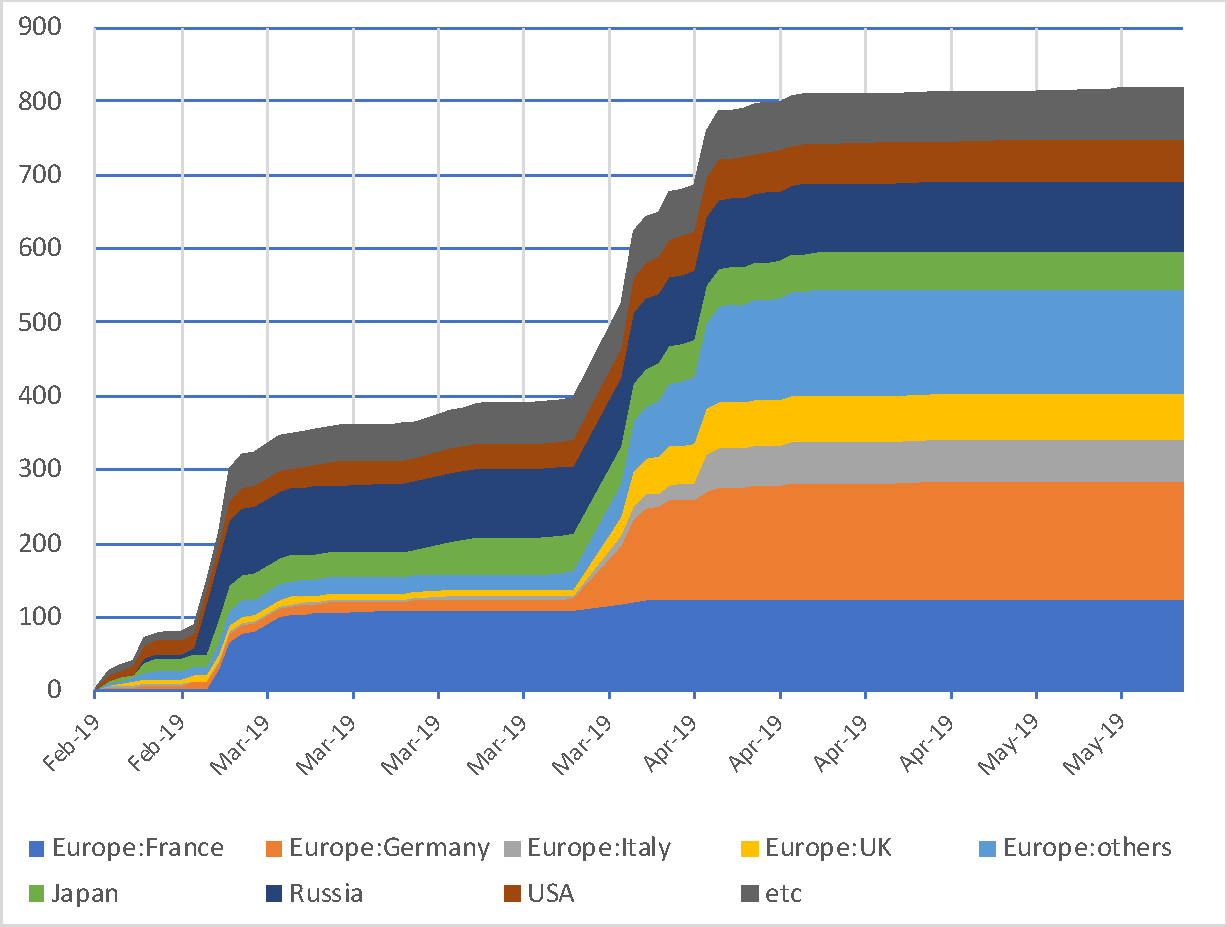
\includegraphics[width=7cm]{Figs/TimeSeries-Zoom.pdf}
\caption{Time series}
\label{fig:time-series}
\end{center}
\end{figure}
%
Unfortunately, this local distribution strategy did not work
universally. Table~\ref{tab:countries} shows the number of
participants of top 11 countries in our survey. In this report, the
countries having more than 50 participants are called {\it major
  countries}. 
Comparing with Table~\ref{tab:top500-share} listing the top 10
countries in the performance share in the Top500\cite{Top500}, the
three major countries, USA, China and Japan, are not even the top 5 in
out survey. Especially China has only 18 participants including
Taiwan. We tried to increase the number of participants of those
countries, especially China, as much as we could, but we failed. Once
we asked a Chinese researcher why we could not get participants from
China and his answer was because of the nationality. 
%
\begin{table}[htb]%
\scriptsize
\begin{center}%
\begin{tabular}[t]{cc}
%
\begin{minipage}[t]{0.5\hsize}
\begin{center}%
\caption{Top 10 Countries of Participants}%
\label{tab:countries}%
\begin{tabular}{c|l|r|r}%
\hline%
\# & Country & \#Ans & [\%] \\%
\hline%
1 & Germany 	& 159 & 18.7 \\%
2 & France 	& 125 & 14.7 \\%
3 & Russia 	& 94  & 11.1 \\%
4 & UK 		& 67  &  7.9 \\%
5 & Japan 	& 64  &  7.5 \\%
6 & USA 	& 58  &  6.8 \\%
7 & Italy 	& 57  &  6.6 \\%
\hline%
8 & Switzerland & 40  &  5.8 \\%
9 & South Korea & 27  &  3.2 \\%
10 & Austria 	& 26  &  3.1 \\%
11 & China (+Taiwan) & 18 & 2.1 \\%
\hline%
\multicolumn{4}{c}{42 countries, 851 participants} \\%
\end{tabular}%
\end{center}%
\end{minipage}
%
\begin{minipage}[t]{0.5\hsize}
\begin{center}%
\caption{Top500 Performance Share (June 2020)\cite{Top500}}%
\label{tab:top500-share}%
\begin{tabular}{c|l|r}%
\hline%
\# & Country & [\%] \\%
\hline%
1  & USA 	  & 28.2 \\%
2  & China 	  & 25.6 \\%
3  & Japan 	  & 23.9 \\%
4  & Italy	  & 4.0  \\%
5  & France	  & 3.6  \\%
6  & Germany 	  & 3.1  \\%
7  & UK		  & 1.4  \\%
8  & Canada	  & 1.3  \\%
9  & Netherlands  & 1.1  \\%
10 & Switzerland  & 1.1  \\%
\hline%
\end{tabular}%
\end{center}%
\end{minipage}%
%
\end{tabular}%
\end{center}%
\end{table}%
%
% Profile
%

\begin{figure}[htb]
\begin{center}
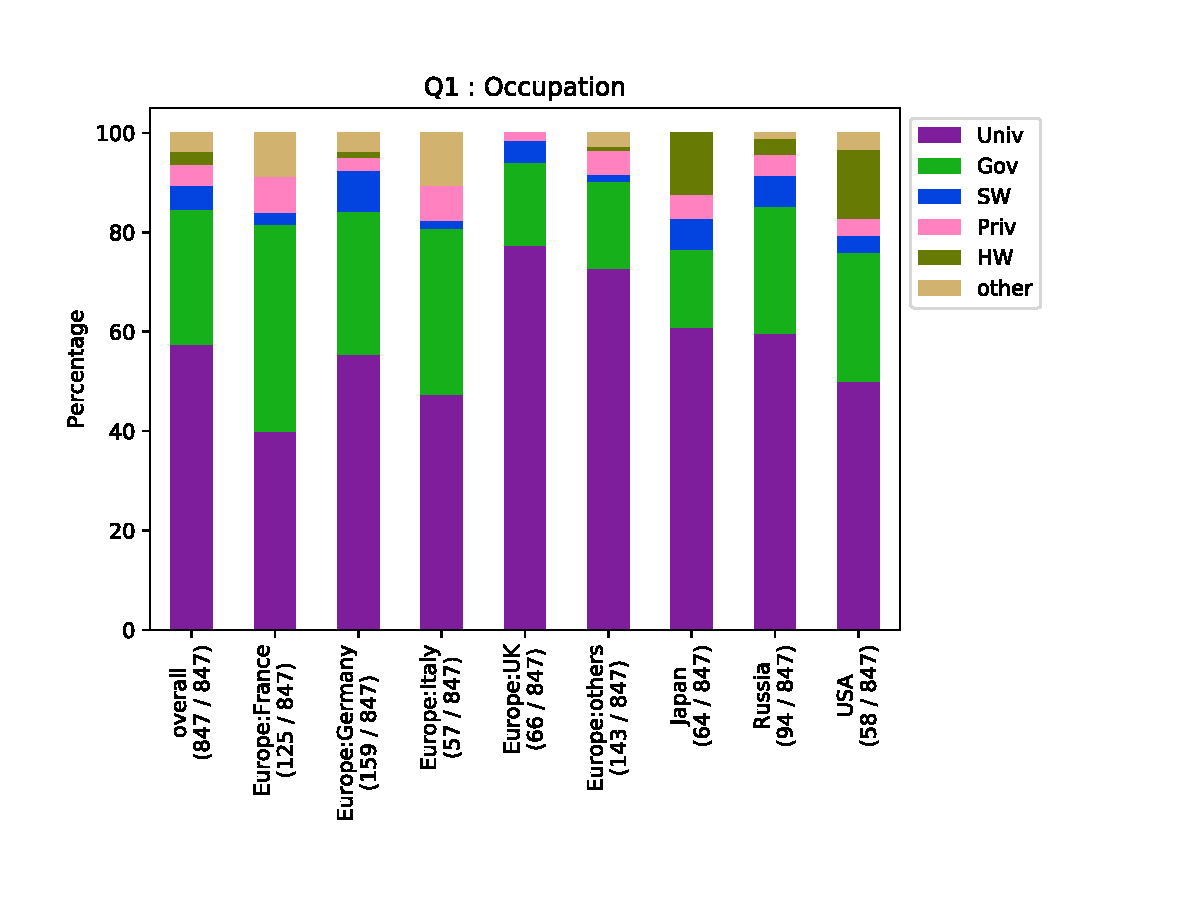
\includegraphics[width=8cm]{Figs/Q1-enlarged.pdf}
\caption{Occupation}
\label{fig:occupation}
\end{center}
\end{figure}

\section{Comparison with the ECP survey}

Although the ECP questionnaire and our questionnaire were designed
independently, there are several questions quite similar in them. 
In the following subsections, we will discuss on those questions, but
before going into the details, we clarify an aspect of US 
participants in our survey.

\begin{figure}[htb]
\begin{center}
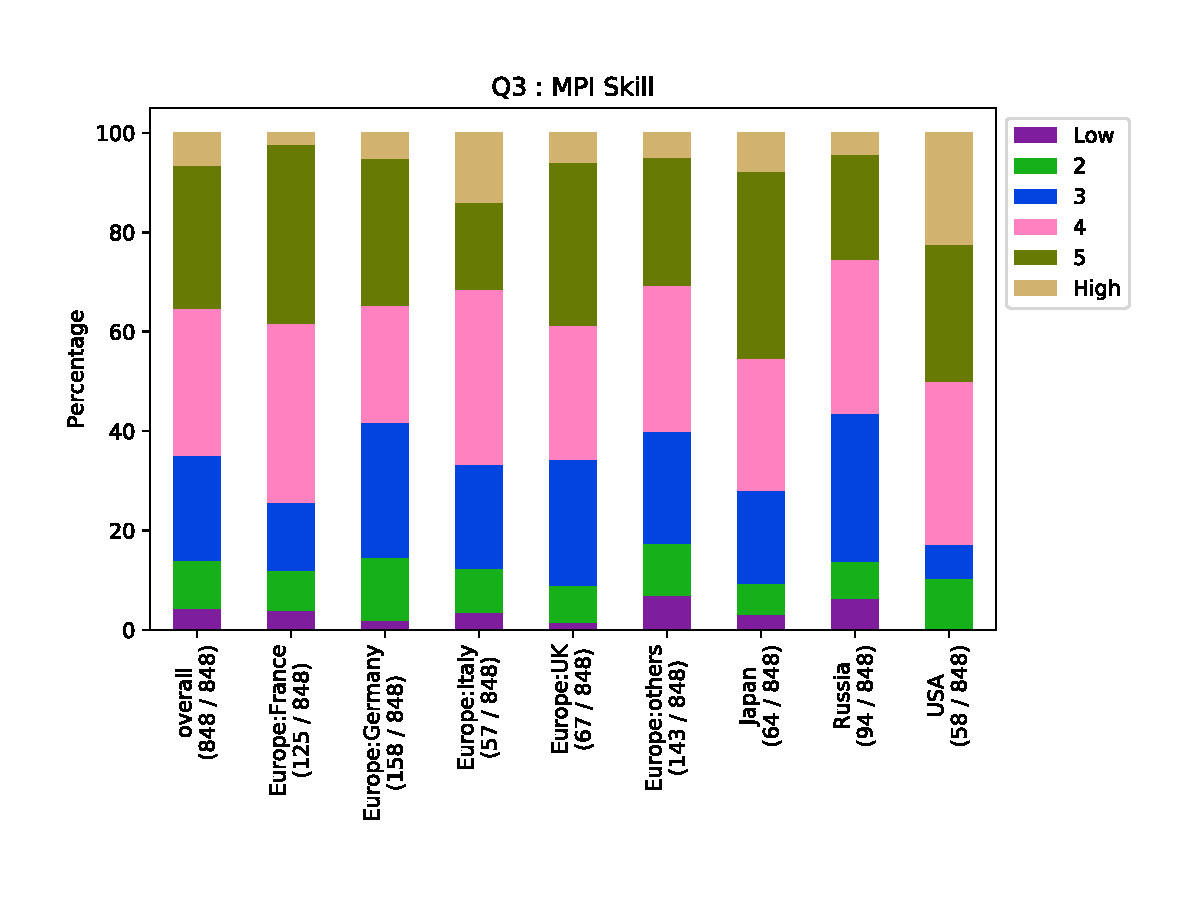
\includegraphics[width=8cm]{Figs/Q3-enlarged.pdf}
\caption{Q3: MPI Skill}
\label{fig:mpi-skill}
\end{center}
\end{figure}

We assumed that the participants in the ECP survey have good
experiences on programming and MPI usage. Fig.~\ref{fig:mpi-skill}
shows the results of Q3 asking to rate participants MPI skill by
themselves in our survey.  In the US case\footnote{Note that we asked
  the workplace in past 5 years, not asking nationalities.} (right
most), almost half of participants rate themselves 5 or 6
(High). This percentage of having high MPI skill ($>=5$) in the US is
the highest among the other countries.

\subsection{Layering MPI calls}

The question in the ECP survey asking ``Do you have an abstraction
layer that hides the MPI calls? Or do most of your developers write
MPI calls directly?'' may correspond to our Q21 asking ``In most of
your programs, do you pack MPI function calls into their own file or
files to have your own abstraction layer for communication?'' 

\begin{figure}[htb]
\begin{center}
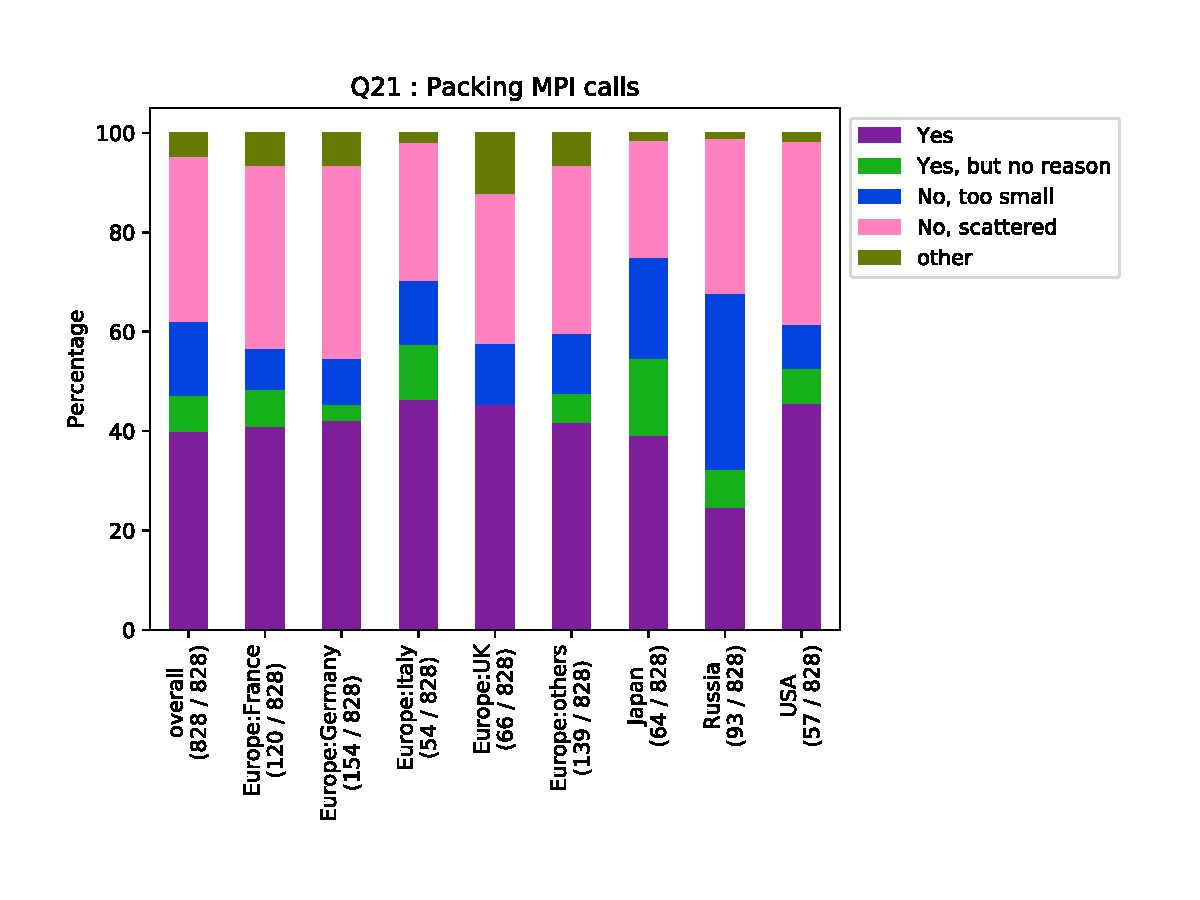
\includegraphics[width=8cm]{Figs/Q21-enlarged.pdf}
\caption{Q21: Layering MPI calls}
\label{fig:layering-mpi-calls}
\end{center}
\end{figure}

\begin{table}[htb]%
\begin{center}%
\caption{Layering MPI calls}\label{tab:layering-mpi-calls}%
\begin{tabular}{c|c||c|c||c}%
\hline%
\multicolumn{2}{c||}{Choice} & \multicolumn{2}{c||}{Our Survey} & ECP \\
\cline{2-5}%
 & Sub-choice & Overall [\%] & USA [\%] & [\%] \\
\hline%
\hline%
Yes & - & 40 & 46 & 62 \\
%\cline{1-4}%
& no reason & 7 & 7 & \\
\hline%
No & too small & 15 & 9 & 38 \\
%\cline{1-4}%
& - & 33 & 37 &  \\
\hline%
Other & - & 5 & 2 & - \\
\hline%
\end{tabular}%
\end{center}%
\end{table}%

\subsection{Using MPI Aspects}

\begin{figure}[htb]
\begin{center}
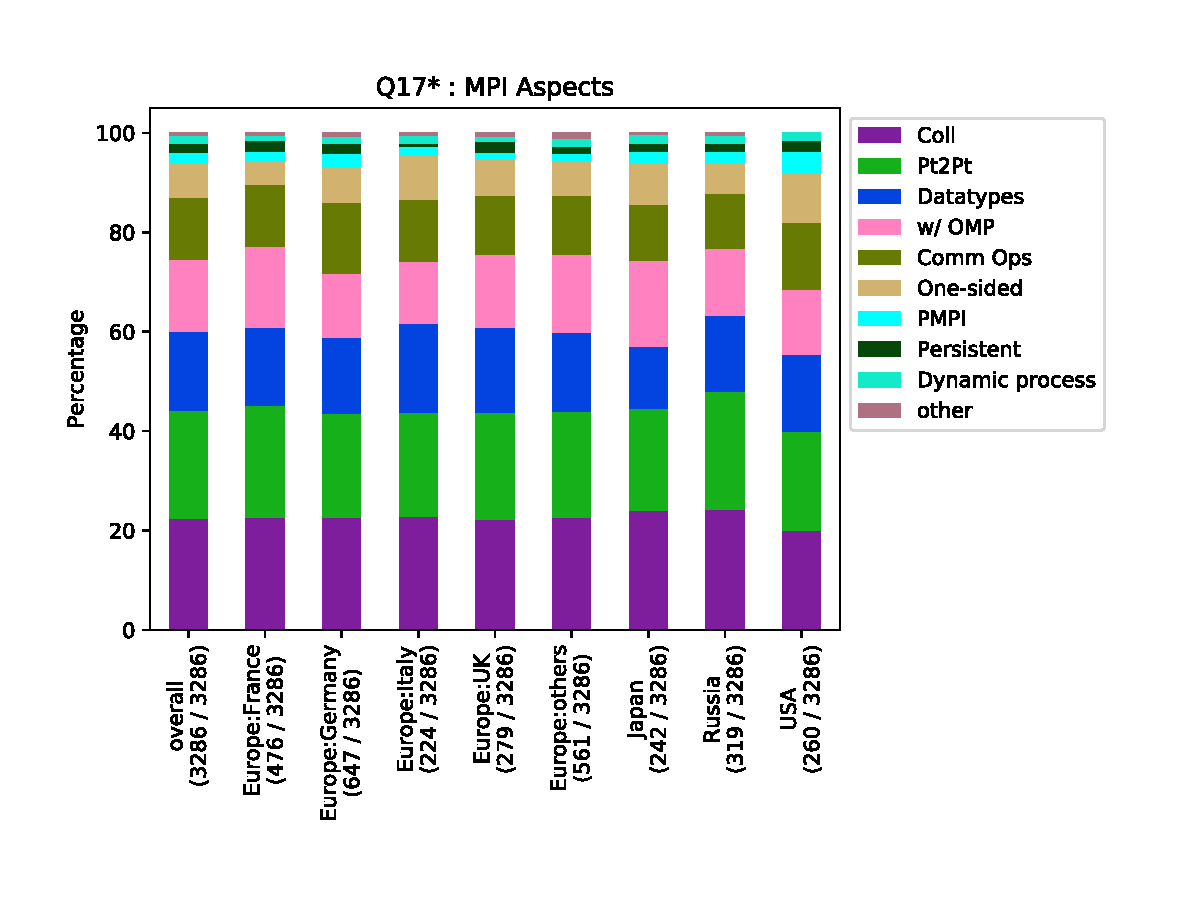
\includegraphics[width=8cm]{Figs/Q17-enlarged.pdf}
\caption{Q17: Using MPI Aspects}
\label{fig:using-mpi-aspects}
\end{center}
\end{figure}

\begin{table}[htb]%
\begin{center}%
\caption{Using MPI Aspects}\label{tab:using-mpi-aspects}%
\begin{tabular}{c||c|c||c}%
\hline%
Choice & \multicolumn{2}{c||}{Our Survey} & ECP \\
\cline{2-4}%
& Overall [\%] & USA [\%] & [\%] \\
\hline%
\hline%
Pt2Pt & 85 & 90 & 88 \\
Datatype & 63 & 69 & 23 \\
Collective & 89 & 90 & 80 \\
Communicator & 50 & 60 & 61 \\
One-sided (RMA) & 27 & 45 & 21 \\
PMPI & 8 & 19 & 14 \\
\hline%
\end{tabular}%
\end{center}%
\end{table}%

\subsection{Multi-Threading}

\begin{figure}[htb]
\begin{center}
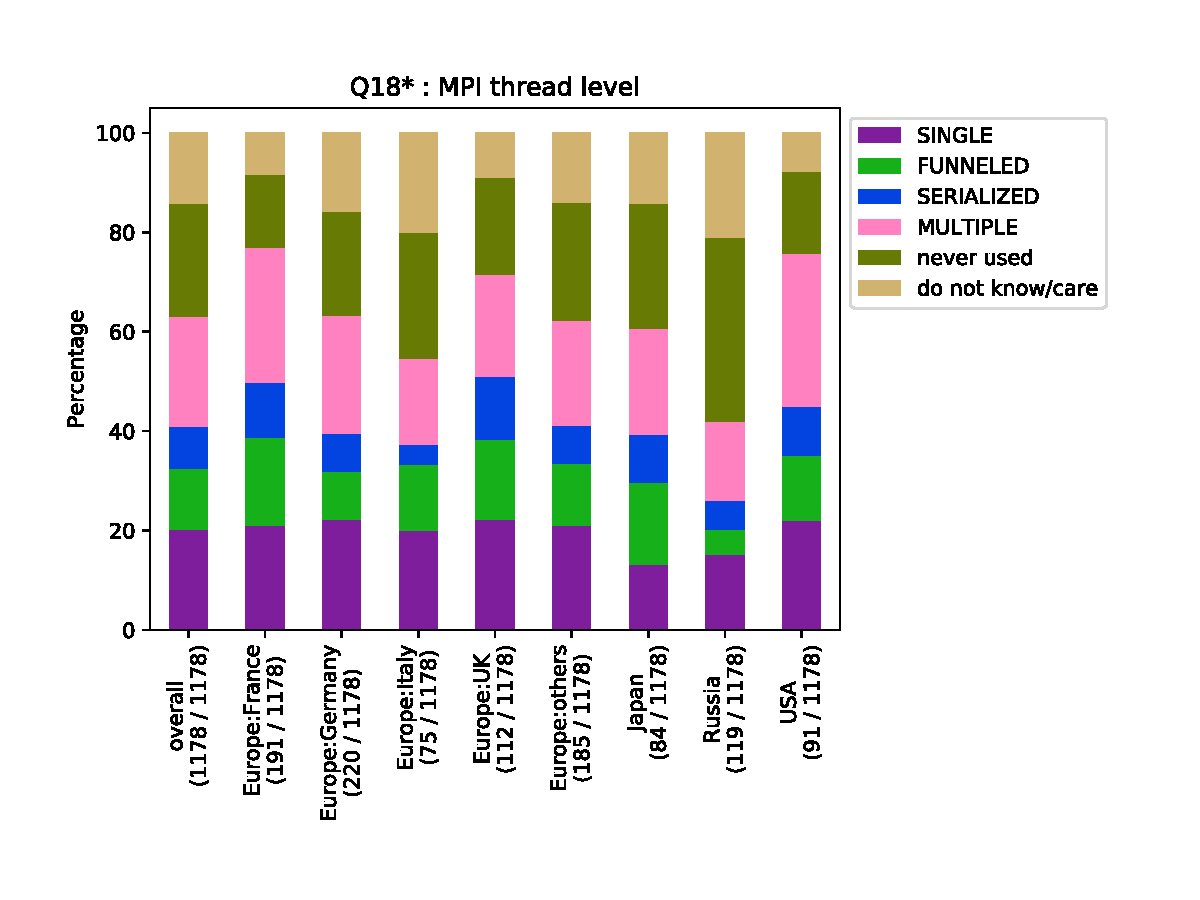
\includegraphics[width=8cm]{Figs/Q18-enlarged.pdf}
\caption{Q18: Multi-Threding}
\label{fig:multi-thread}
\end{center}
\end{figure}

\begin{table}[htb]%
\begin{center}%
\caption{Multi-Threading}\label{tab:multi-thread}%
\begin{tabular}{c||c|c||c}%
\hline%
Choice & \multicolumn{2}{c||}{Our Survey} & ECP \\
\cline{2-4}%
& Overall [\%] & USA [\%] & [\%] \\
\hline%
\hline%
SINGLE & 29 & 22 & - \\
FUNNELED & 18 & 13 & 18 \\
SERIALIZED & 12 & 10 & 18 \\
MULTIPLE & 22 & 31 & 25 \\
never & 23 & 16 & - \\
not know & 14 & 8 & 25 \\
\hline%
\end{tabular}%
\end{center}%
\end{table}%


\subsection{Multi-threading}


\section{Other Findings}

\subsection{Skill}

\subsection{New Features}

\subsection{Compatibility vs. Performance}

\section{Summary}

\section*{Acknowledgments}
We thank to those who participated in this survey and those who
helped us to distribute the questionnaire to their local
communities. We especially thank to MPI Forum members who gave us many
significant comments on the draft questionnaire.
This research is partially supported by the
NCSA-Inria-ANL-BSC-JSC-Riken-UTK Joint-Laboratory for Extreme Scale
Computing~\cite{JLESC}.

\bibliographystyle{IEEEtran}
\bibliography{../ref}

\end{document}
